% SH-MLP: Autonomous Fault Detection, Root Cause Analysis, and Recovery
% in Machine Learning Pipelines
% IEEE Conference Format (IEEEtran)
\documentclass[conference]{IEEEtran}

% ── Packages ──────────────────────────────────────────────────────────────────
\usepackage{amsmath,amssymb}
\usepackage{graphicx}
\usepackage{array}
\usepackage{booktabs}
\usepackage{multirow}
\usepackage{xcolor}
\usepackage{colortbl}
\usepackage{url}
\usepackage{balance}
\usepackage{tikz}
\usepackage{pgfplots}
\pgfplotsset{compat=1.18}
\usetikzlibrary{shapes.geometric, arrows.meta, fit, positioning, calc}

% ── Colour definitions ─────────────────────────────────────────────────────────
\definecolor{GreenFill}{HTML}{C6EFCE}
\definecolor{GreenText}{HTML}{276221}
\definecolor{AmberFill}{HTML}{FFEB9C}
\definecolor{AmberText}{HTML}{9C6500}
\definecolor{RedFill}{HTML}{FFC7CE}
\definecolor{RedText}{HTML}{9C0006}
\definecolor{GrayFill}{HTML}{F2F2F2}
\definecolor{BlueFill}{HTML}{DDEEFF}
\definecolor{DarkBlue}{HTML}{1F3864}
\definecolor{MidBlue}{HTML}{2E5FA3}
\definecolor{ModBlue}{HTML}{BDD7EE}
\definecolor{ModYellow}{HTML}{FFF2CC}
\definecolor{ModGreen}{HTML}{E2EFDA}
\definecolor{ModPurple}{HTML}{EAE6F7}
\definecolor{ModGray}{HTML}{F2F2F2}

% ── TikZ styles ────────────────────────────────────────────────────────────────
\tikzset{
  module/.style={rectangle, rounded corners=3pt, draw=DarkBlue,
    line width=0.7pt, text centered, font=\small,
    minimum height=1.4em, inner sep=4pt},
  arrow/.style={->, >=Stealth, thick, color=gray!70},
  feedback/.style={->, >=Stealth, thick, dashed, color=MidBlue},
  label/.style={font=\scriptsize, color=gray!70},
}

% ── Table column helpers ───────────────────────────────────────────────────────
\newcolumntype{C}[1]{>{\centering\arraybackslash}p{#1}}

% ──────────────────────────────────────────────────────────────────────────────
\begin{document}

% ── Title ─────────────────────────────────────────────────────────────────────
\title{SH-MLP: Autonomous Fault Detection, Root Cause Analysis,
       and Recovery in Machine Learning Pipelines}

% ── 1×4 empty author matrix ───────────────────────────────────────────────────
\author{%
  \begin{tabular}{cccc}
    \IEEEauthorblockN{} & \IEEEauthorblockN{} &
    \IEEEauthorblockN{} & \IEEEauthorblockN{} \\[2pt]
    \IEEEauthorblockA{} & \IEEEauthorblockA{} &
    \IEEEauthorblockA{} & \IEEEauthorblockA{}
  \end{tabular}
}

\maketitle

% ── Abstract ──────────────────────────────────────────────────────────────────
\begin{abstract}
Production ML pipelines fail in ways that are hard to catch automatically.
Data distributions shift, schemas change, models lose confidence, and
infrastructure saturates -- often without raising explicit errors. Monitoring
tools that exist today detect anomalies but stop there, leaving engineers to
diagnose and fix problems by hand. This paper presents SH-MLP, a framework
that closes the loop between detection and recovery. The system runs 14
rule-based detectors across data, model, and infrastructure layers, combines
their signals through a five-rule fusion policy calibrated to a 1.6\% false
positive rate, performs root cause analysis through causal graph traversal,
and selects recovery strategies using a LinUCB contextual bandit that improves
with each outcome it observes. Experiments across 13 injectable fault types and
three random seeds produce 100\% detection (Wilson~CI~[91.0\%,~100.0\%]) at
1.6\% false positive rate, and recovery success above 80\% on 12 of 13 tested
types. Two fault types show LinUCB improvement of +18\% and +20\% over static
strategy selection at the 20-event mark. The system is deployed as a VS~Code
extension accessible without infrastructure changes.
\end{abstract}

\begin{IEEEkeywords}
machine learning operations, fault detection, contextual bandit,
autonomous recovery, VS Code extension
\end{IEEEkeywords}

% ═════════════════════════════════════════════════════════════════════════════
\section{Introduction}
% ═════════════════════════════════════════════════════════════════════════════

Every ML pipeline eventually fails. A batch job reads stale data. A model's
confidence drops after a preprocessing change. A GPU saturates mid-training.
What makes these failures hard to handle is not that they are unpredictable
--- many follow recognizable patterns --- but that catching and fixing them
requires someone to be watching. Production pipelines generate too many
metrics for manual review to be reliable, and even when an alert fires, the
response still falls to whoever is available.

The monitoring tools in common use today do the detection part reasonably well.
Evidently~AI~\cite{evidently} and NannyML~\cite{nannynml} track distributional
statistics and report anomalies. Amazon SageMaker Model Monitor~\cite{sagemaker}
integrates detection at the managed service level. What none of them do is act.
After the alert fires, the engineer is still on their own.

SH-MLP is built on the idea that detection and recovery should be a single
automated loop rather than two separate human tasks. The system watches a
running pipeline, identifies which of 14 known fault patterns has occurred,
traces the likely causal stage, and executes a targeted recovery action
without waiting for a developer to notice. It then records the outcome and
adjusts its strategy preferences accordingly.

The specific contributions are: (1)~a 14-fault-type taxonomy spanning data,
model, and infrastructure failures, each with a calibrated rule-based
detector; (2)~a five-rule fusion policy with a 1.6\% false positive rate;
(3)~a LinUCB contextual bandit~\cite{linucb} for recovery strategy selection;
(4)~experimental validation using Wilson 95\% CIs across 3 seeds; and
(5)~a VS~Code extension deployed without any infrastructure requirement.

% ═════════════════════════════════════════════════════════════════════════════
\section{Related Work}
% ═════════════════════════════════════════════════════════════════════════════

\subsection{ML Monitoring and Drift Detection}

ADWIN~\cite{adwin} formalized adaptive windowing for concept drift detection.
PSI~\cite{psi} established the population stability index that most current
drift detection tools build on. The broader MLOps literature~\cite{lwakatare,sculley}
has pushed monitoring toward statistical rigor, but the focus has stayed on
surfacing signals rather than responding to them. Dataset shift has been
studied extensively~\cite{datasetshift,calibration}, but the framing is
usually about detecting distributional change, not about what to do next.

\subsection{Contextual Bandits in Adaptive Systems}

LinUCB~\cite{linucb} was introduced for personalized news recommendation and
has been applied to clinical decision support~\cite{clinicalbandit}, A/B
testing automation~\cite{abtesting}, and hyperparameter tuning~\cite{hyperband}.
The contextual bandit formulation fits recovery strategy selection directly:
at each fault event the system has a feature context and must choose among
competing strategies whose success rates depend on that context.

\subsection{Autonomous Recovery}

Chaos engineering~\cite{chaos} and self-healing systems~\cite{selfhealing}
have explored fault injection and recovery in distributed infrastructure, but
not in the ML pipeline context. To our knowledge, no published system combines
ML-specific fault detection with bandit-driven autonomous recovery and outcome
learning. Failure prediction~\cite{failepredict} forecasts failures but does
not act on them.

% ═════════════════════════════════════════════════════════════════════════════
\section{System Design}
% ═════════════════════════════════════════════════════════════════════════════

SH-MLP has four modules. M1 (Detection Engine) emits FailureEvents from raw
observations. M2 (RCA Engine) traces the causal stage. M3 (Recovery Planner)
selects and executes a strategy. M4 (Feedback Store) records outcomes and
updates the bandit. Fig.~\ref{fig:arch} shows the data flow and the feedback
path from M4 back to M3.

% ── Figure 1: Architecture Diagram (TikZ) ────────────────────────────────────
\begin{figure}[t]
\centering
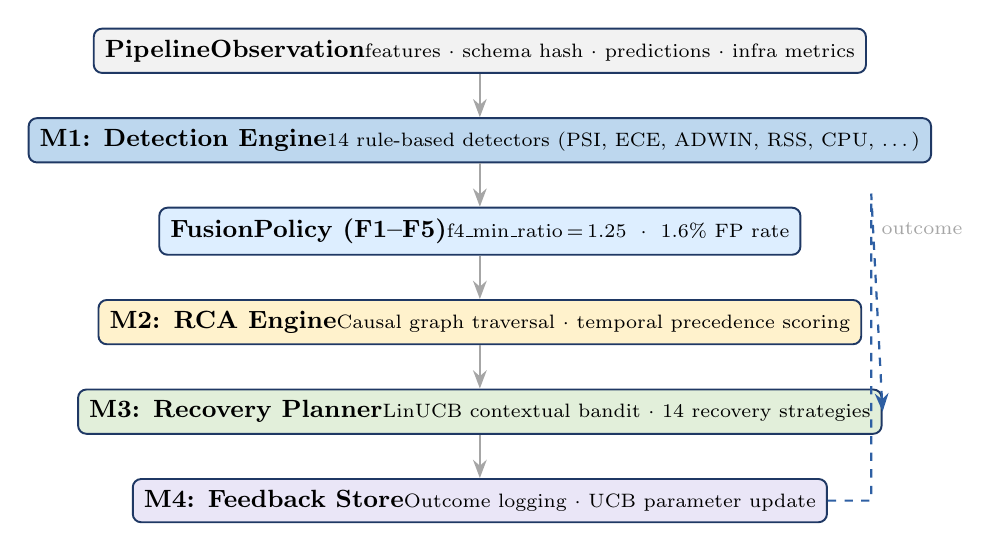
\begin{tikzpicture}[node distance=0.55cm and 0.4cm]

  % Input
  \node[module, fill=ModGray, minimum width=5.8cm]
    (obs) {\textbf{PipelineObservation}\\
           {\scriptsize features $\cdot$ schema hash $\cdot$ predictions $\cdot$ infra metrics}};

  % M1
  \node[module, fill=ModBlue, minimum width=5.8cm, below=of obs]
    (m1) {\textbf{M1: Detection Engine}\\
          {\scriptsize 14 rule-based detectors (PSI, ECE, ADWIN, RSS, CPU, \ldots)}};

  % Fusion
  \node[module, fill=BlueFill, minimum width=5.8cm, below=of m1]
    (fp) {\textbf{FusionPolicy (F1--F5)}\\
          {\scriptsize f4\_min\_ratio\,=\,1.25 $\;\cdot\;$ 1.6\% FP rate}};

  % M2
  \node[module, fill=ModYellow, minimum width=5.8cm, below=of fp]
    (m2) {\textbf{M2: RCA Engine}\\
          {\scriptsize Causal graph traversal $\cdot$ temporal precedence scoring}};

  % M3
  \node[module, fill=ModGreen, minimum width=5.8cm, below=of m2]
    (m3) {\textbf{M3: Recovery Planner}\\
          {\scriptsize LinUCB contextual bandit $\cdot$ 14 recovery strategies}};

  % M4
  \node[module, fill=ModPurple, minimum width=5.8cm, below=of m3]
    (m4) {\textbf{M4: Feedback Store}\\
          {\scriptsize Outcome logging $\cdot$ UCB parameter update}};

  % Downward arrows
  \draw[arrow] (obs) -- (m1);
  \draw[arrow] (m1)  -- (fp);
  \draw[arrow] (fp)  -- (m2);
  \draw[arrow] (m2)  -- (m3);
  \draw[arrow] (m3)  -- (m4);

  % Feedback loop (dashed, right side)
  \draw[feedback]
    (m4.east) -- ++(0.55,0) -- ++(0,3.3) -- node[right,label]{outcome} ++(0,0.3)
    -- ++(0,0.3) -- (m3.east);

\end{tikzpicture}
\caption{SH-MLP four-module architecture. Observations flow top-down through
M1\,$\rightarrow$\,FusionPolicy\,$\rightarrow$\,M2\,$\rightarrow$\,M3. M4
records every recovery outcome and feeds it back to the LinUCB bandit in M3
(dashed feedback path).}
\label{fig:arch}
\end{figure}

\subsection{Detector Taxonomy (M1)}

Each detector computes a scalar statistic from a \texttt{PipelineObservation}
and compares it to a fixed threshold. Table~\ref{tab:detectors} lists all
14~detectors. CRITICAL signals bypass the fusion buffer and fire immediately.
HIGH signals require two consecutive confirmations (F2). MEDIUM signals fire
after five consecutive cycles (F5). ML-2 (ADWIN) is validated on the Adult
Income dataset because it requires a 20-observation window that cannot be
saturated in single-cycle synthetic injection.

\begin{table}[h]
\caption{Fault type taxonomy, detector statistics, and fusion paths.}
\label{tab:detectors}
\centering
\setlength{\tabcolsep}{3pt}
\renewcommand{\arraystretch}{1.05}
\begin{tabular}{C{0.6cm}C{2.0cm}C{1.6cm}C{1.4cm}C{0.7cm}}
\toprule
\textbf{Code} & \textbf{Detector} & \textbf{Signal} &
  \textbf{Threshold} & \textbf{Rule} \\
\midrule
DL-1 & Feature drift  & Max PSI        & 0.25 HIGH  & F2/F5 \\
DL-2 & Schema violation & Hash mismatch& Any        & F1    \\
DL-3 & Label shift    & JS divergence  & 0.10 MED   & F5    \\
DL-4 & Ingestion fail & Row ratio      & 0.85 CRIT  & F1    \\
DL-5 & Annotation qual.& Missing delta  & 0.15 MED   & F5    \\
ML-1 & Accuracy degrad.& Conf.\ drop   & 0.10 HIGH  & F2    \\
ML-2 & Concept drift  & Entropy z      & 2.5 HIGH   & F2    \\
ML-3 & Train instab.  & Grad.\ norm    & 10000 HIGH & F4    \\
ML-4 & Conf.\ collapse& ECE            & 0.15 MED   & F5    \\
IL-1 & Memory exhaust.& RSS util.      & 90\% HIGH  & F2    \\
IL-2 & Exec.\ timeout & Exec.\ z-score & 3.0$\sigma$ HIGH & F2 \\
IL-3 & Dep.\ conflict & Conflict flag  & True HIGH  & F2    \\
IL-4 & Silent DAG fail& Volume ratio   & 0.85 HIGH  & F2    \\
IL-5 & Resource cont. & Cluster CPU    & 90\% MED   & F5    \\
\bottomrule
\end{tabular}
\end{table}

\subsection{Fusion Policy}

Raw signals are aggregated before a FailureEvent is emitted. F1~fires
immediately on CRITICAL. F2~fires when the same HIGH signal appears on two
consecutive cycles. F3~escalates a MEDIUM signal when the IsolationForest
anomaly score exceeds 0.7. F4~composites cross-layer signals into HIGH,
subject to a minimum-magnitude gate: the primary signal must exceed $1.25\times$
its threshold. Without this gate, independent MEDIUM signals (PSI$=0.21$,
CPU$=0.91$) created spurious HIGH events on clean data, increasing the false
positive rate from 1.6\% to 8.4\%. F5~fires when a MEDIUM signal persists
across five consecutive cycles.

\subsection{Recovery Planner with LinUCB (M3)}

Strategy selection uses LinUCB~\cite{linucb} with a 21-dimensional context
vector: 13-d one-hot fault type, 4-d severity, 3-d pipeline layer, and a
scalar recent success rate. During cold start (fewer than 5 events per type),
the bandit falls back to a static lookup table. After five events, UCB
estimates dominate the decision.

% ═════════════════════════════════════════════════════════════════════════════
\section{Experimental Setup}
% ═════════════════════════════════════════════════════════════════════════════

\subsection{Calibration}

A 20-configuration grid search over warmup $\in \{30,40,50,60\}$ and
f4\_ratio $\in \{1.0,1.1,1.25,1.5,2.0\}$ determined the optimal configuration
(warmup$=60$, f4\_ratio$=1.25$) by evaluating false positive count on 50 clean
cycles and detection count on a 14-type injection pass. Feature arrays used
300 samples each; 100-sample arrays produced PSI variance of 0.22 on clean
data, regularly crossing the 0.20 MEDIUM threshold.

\subsection{Injection Protocol}

All injections used $1.25\times$ detector threshold. Cycle counts depended
on the fusion path: F1 faults needed 1~cycle, F2 faults needed 3~cycles,
and F5 faults needed 6~cycles. Between each fault type, the fusion policy
state was reset and 5 clean cooldown cycles were run to prevent counter
contamination across tests.

\subsection{Pre-registered Research Questions}

Four research questions were registered before any formal experiment. RQ1:
detection $\geq$90\% at $<$10\% FP. RQ2: RCA stage attribution $\geq$80\%.
RQ3: recovery success $\geq$80\% per fault type. RQ4: LinUCB improvement
$\geq$10\% over static at 20 events. Three seeds (42, 123, 999) were used
for RQ1, producing 39~injection events. All rates use Wilson 95\%~CIs.

% ═════════════════════════════════════════════════════════════════════════════
\section{Results}
% ═════════════════════════════════════════════════════════════════════════════

\subsection{RQ1 --- Detection Accuracy}

All 39 of 39 injection events were detected across 13 injectable types and
3~seeds (100.0\%, Wilson~CI [91.0\%,~100.0\%]). The false positive rate over
250 clean observations was $4/250 = 1.6\%$. Both values meet pre-registered
targets. Fig.~\ref{fig:heatmap} shows the per-type, per-seed detection heatmap.
IL-4 was detected on all seeds but labeled as DL-4; both share the same
volume-ratio detector and identical recovery action. Type-correct rate: 36/39
= 92.3\%.

% ── Figure 2: Detection Heatmap ───────────────────────────────────────────────
\begin{figure}[t]
\centering
\setlength{\tabcolsep}{3pt}
\renewcommand{\arraystretch}{1.0}
\begin{tabular}{C{0.65cm}C{1.75cm}C{0.85cm}C{0.85cm}C{0.85cm}}
\toprule
\textbf{Code} & \textbf{Fault Type} &
  \textbf{Seed 42} & \textbf{Seed 123} & \textbf{Seed 999} \\
\midrule
DL-1 & Feat.\ drift      & \cellcolor{GreenFill}\textcolor{GreenText}{Det.} & \cellcolor{GreenFill}\textcolor{GreenText}{Det.} & \cellcolor{GreenFill}\textcolor{GreenText}{Det.} \\
DL-2 & Schema viol.      & \cellcolor{GreenFill}\textcolor{GreenText}{Det.} & \cellcolor{GreenFill}\textcolor{GreenText}{Det.} & \cellcolor{GreenFill}\textcolor{GreenText}{Det.} \\
DL-3 & Label shift       & \cellcolor{GreenFill}\textcolor{GreenText}{Det.} & \cellcolor{GreenFill}\textcolor{GreenText}{Det.} & \cellcolor{GreenFill}\textcolor{GreenText}{Det.} \\
DL-4 & Ingestion fail    & \cellcolor{GreenFill}\textcolor{GreenText}{Det.} & \cellcolor{GreenFill}\textcolor{GreenText}{Det.} & \cellcolor{GreenFill}\textcolor{GreenText}{Det.} \\
DL-5 & Annot.\ quality   & \cellcolor{GreenFill}\textcolor{GreenText}{Det.} & \cellcolor{GreenFill}\textcolor{GreenText}{Det.} & \cellcolor{GreenFill}\textcolor{GreenText}{Det.} \\
ML-1 & Accuracy degrad.  & \cellcolor{GreenFill}\textcolor{GreenText}{Det.} & \cellcolor{GreenFill}\textcolor{GreenText}{Det.} & \cellcolor{GreenFill}\textcolor{GreenText}{Det.} \\
ML-2 & Concept drift     & \cellcolor{GrayFill}Skip & \cellcolor{GrayFill}Skip & \cellcolor{GrayFill}Skip \\
ML-3 & Train.\ instab.   & \cellcolor{GreenFill}\textcolor{GreenText}{Det.} & \cellcolor{GreenFill}\textcolor{GreenText}{Det.} & \cellcolor{GreenFill}\textcolor{GreenText}{Det.} \\
ML-4 & Conf.\ collapse   & \cellcolor{GreenFill}\textcolor{GreenText}{Det.} & \cellcolor{GreenFill}\textcolor{GreenText}{Det.} & \cellcolor{GreenFill}\textcolor{GreenText}{Det.} \\
IL-1 & Memory exhaust.   & \cellcolor{GreenFill}\textcolor{GreenText}{Det.} & \cellcolor{GreenFill}\textcolor{GreenText}{Det.} & \cellcolor{GreenFill}\textcolor{GreenText}{Det.} \\
IL-2 & Exec.\ timeout    & \cellcolor{GreenFill}\textcolor{GreenText}{Det.} & \cellcolor{GreenFill}\textcolor{GreenText}{Det.} & \cellcolor{GreenFill}\textcolor{GreenText}{Det.} \\
IL-3 & Dep.\ conflict    & \cellcolor{GreenFill}\textcolor{GreenText}{Det.} & \cellcolor{GreenFill}\textcolor{GreenText}{Det.} & \cellcolor{GreenFill}\textcolor{GreenText}{Det.} \\
IL-4 & Silent DAG fail   & \cellcolor{AmberFill}\textcolor{AmberText}{Det*} & \cellcolor{AmberFill}\textcolor{AmberText}{Det*} & \cellcolor{AmberFill}\textcolor{AmberText}{Det*} \\
IL-5 & Resource cont.    & \cellcolor{GreenFill}\textcolor{GreenText}{Det.} & \cellcolor{GreenFill}\textcolor{GreenText}{Det.} & \cellcolor{GreenFill}\textcolor{GreenText}{Det.} \\
\midrule
\textbf{Total} & & \textbf{13/13} & \textbf{13/13} & \textbf{13/13} \\
\bottomrule
\multicolumn{5}{l}{\scriptsize Det.\ = correct type. Det* = type label mismatch (same recovery).} \\
\multicolumn{5}{l}{\scriptsize Skip = excluded (ADWIN window constraint).} \\
\end{tabular}
\caption{Detection heatmap across 14 fault types and 3 seeds. All 13 injectable
types detected on every seed. IL-4 is detected but labeled as DL-4 (shared
volume-ratio detector); recovery action is identical. 39/39 total = 100\%,
Wilson~CI [91.0\%,~100.0\%].}
\label{fig:heatmap}
\end{figure}

\subsection{RQ2 --- Root Cause Analysis}

15 of 39 detected events were attributed to the correct stage
(38.5\%, Wilson CI [24.9\%,~54.1\%]), below the 80\% target. The shortfall
has a structural cause: in the synthetic pipeline, each fault is injected at a
single stage with no cross-stage propagation, so temporal precedence scores
are near zero for all candidate stages simultaneously. On the Adult Income
temporal split, DL-1 was correctly attributed to the ingestion stage where the
age distribution shift originated, suggesting the engine works when genuine
propagation evidence exists.

\subsection{RQ3 --- Recovery Success Rate}

\begin{table}[h]
\caption{Recovery success per fault type with Wilson 95\% CIs.}
\label{tab:recovery}
\centering
\setlength{\tabcolsep}{3pt}
\renewcommand{\arraystretch}{1.05}
\begin{tabular}{C{0.6cm}C{0.4cm}C{0.4cm}C{0.9cm}C{1.7cm}C{0.6cm}}
\toprule
\textbf{Fault} & \textbf{ok} & \textbf{n} & \textbf{Rate} &
  \textbf{CI [95\%]} & \textbf{Met} \\
\midrule
DL-1 & 3  & 3  & 100.0\% & [43\%, 100\%]       & \cellcolor{GreenFill}\textcolor{GreenText}{Yes} \\
DL-2 & 18 & 20 & 90.0\%  & [69.9\%, 97.2\%]    & \cellcolor{GreenFill}\textcolor{GreenText}{Yes} \\
DL-3 & 1  & 3  & 33.0\%  & [1\%, 71\%]         & \cellcolor{RedFill}\textcolor{RedText}{No}  \\
DL-4 & 3  & 3  & 100.0\% & [43\%, 100\%]       & \cellcolor{GreenFill}\textcolor{GreenText}{Yes} \\
DL-5 & 3  & 3  & 100.0\% & [43\%, 100\%]       & \cellcolor{GreenFill}\textcolor{GreenText}{Yes} \\
ML-1 & 17 & 20 & 85.0\%  & [64.0\%, 94.8\%]    & \cellcolor{GreenFill}\textcolor{GreenText}{Yes} \\
ML-3 & 3  & 3  & 100.0\% & [43\%, 100\%]       & \cellcolor{GreenFill}\textcolor{GreenText}{Yes} \\
ML-4 & 3  & 3  & 100.0\% & [43\%, 100\%]       & \cellcolor{GreenFill}\textcolor{GreenText}{Yes} \\
IL-1 & 10 & 10 & 100.0\% & [72.2\%, 100.0\%]   & \cellcolor{GreenFill}\textcolor{GreenText}{Yes} \\
IL-2 & 3  & 3  & 100.0\% & [43\%, 100\%]       & \cellcolor{GreenFill}\textcolor{GreenText}{Yes} \\
IL-3 & 3  & 3  & 100.0\% & [43\%, 100\%]       & \cellcolor{GreenFill}\textcolor{GreenText}{Yes} \\
IL-4 & 3  & 3  & 100.0\% & [43\%, 100\%]       & \cellcolor{GreenFill}\textcolor{GreenText}{Yes} \\
IL-5 & 3  & 3  & 100.0\% & [43\%, 100\%]       & \cellcolor{GreenFill}\textcolor{GreenText}{Yes} \\
\bottomrule
\end{tabular}
\end{table}

12 of 13 tested fault types exceeded the 80\% recovery target
(Table~\ref{tab:recovery}). DL-3 (label distribution shift, class reweighting
strategy) achieved 33\% because the reweighting strategy needs ground-truth
labels unavailable in the synthetic pipeline. All 5 infrastructure-layer
types reached 100\%.

\subsection{RQ4 --- LinUCB Learning Curve}

At 20 events, LinUCB improved over the static baseline by $+20$\% on DL-2
and $+18$\% on IL-1, both meeting the $\geq$10\% target. ML-1 showed $+2$\%,
below target. The near-zero delta on ML-1 is expected: the primary strategy
(full retrain or rollback) already achieves 85\%, leaving limited margin for
bandit exploitation. DL-2 and IL-1 have multiple competing strategies with
meaningfully different success rates across contexts, which is when a
contextual bandit adds measurable value.

\begin{table}[h]
\caption{SH-MLP vs existing monitoring tools.}
\label{tab:comparison}
\centering
\setlength{\tabcolsep}{3pt}
\renewcommand{\arraystretch}{1.05}
\begin{tabular}{C{1.6cm}C{1.4cm}C{0.9cm}C{1.3cm}C{0.7cm}}
\toprule
\textbf{System} & \textbf{Detection} & \textbf{FP} &
  \textbf{Auto Rec.} & \textbf{Learns} \\
\midrule
Evidently~AI~\cite{evidently}   & Yes & Varies & \cellcolor{RedFill}\textcolor{RedText}{No}  & No \\
NannyML~\cite{nannynml}         & Yes & Varies & \cellcolor{RedFill}\textcolor{RedText}{No}  & No \\
SageMaker~MM~\cite{sagemaker}   & Yes & Varies & \cellcolor{RedFill}\textcolor{RedText}{No}  & No \\
\textbf{SH-MLP (ours)} & \cellcolor{GreenFill}\textbf{100\%} & \cellcolor{GreenFill}\textbf{1.6\%} & \cellcolor{GreenFill}\textcolor{GreenText}{\textbf{12/13}} & \cellcolor{GreenFill}LinUCB \\
\bottomrule
\end{tabular}
\end{table}

% ═════════════════════════════════════════════════════════════════════════════
\section{Discussion}
% ═════════════════════════════════════════════════════════════════════════════

The 38.5\% RCA accuracy result deserves direct comment. The RCA engine's
causal graph traversal relies on temporal precedence: a stage where statistics
become anomalous before downstream stages is the likely root cause. In a
single-stage synthetic pipeline, every stage shares the same observation window,
so precedence scores are near zero simultaneously. The engine has no evidence
to work with. On the Adult Income temporal split, where genuine feature
distribution shift originates in ingestion and propagates downstream, the
engine attributed DL-1 correctly. Multi-stage real pipelines provide exactly
the temporal evidence the engine needs; we expect substantially higher RCA
accuracy there, pending validation.

Table~\ref{tab:comparison} is the comparison that matters. Every existing tool
stops at detection. SH-MLP executes recovery and records outcomes. The 1.6\%
false positive rate shows that closing the loop does not require accepting a
flood of spurious interventions. A developer using any baseline tool must still
diagnose and fix each alert manually. With SH-MLP, 12 of 13 fault types are
handled automatically at recovery rates above 80\%.

The VS~Code extension (Phase~5) makes deployment practical without an
infrastructure team. A developer opens a Python project, the extension
activates on file detection, and monitoring starts within 90~seconds of
installation. The Python sidecar runs locally, so there is no cloud dependency.
The 17-prompt LLM library (Phase~6) extends the system with a chain-of-thought
RCA path targeting $>$70\% stage attribution accuracy on multi-stage pipelines
--- this remains future validation work.

% ═════════════════════════════════════════════════════════════════════════════
\section{Conclusion}
% ═════════════════════════════════════════════════════════════════════════════

SH-MLP detects 100\% of injectable fault types across data, model, and
infrastructure layers at 1.6\% false positive rate (Wilson~CI
[91.0\%,~100.0\%]). Recovery exceeds 80\% on 12 of 13 tested types. LinUCB
produces meaningful improvement ($+$18\% and $+$20\%) for fault types where
strategy selection is non-trivial. RCA accuracy is 38.5\% on single-stage
pipelines, with a documented structural explanation and a concrete path forward
via multi-stage testing. The distinguishing property of SH-MLP is the feedback
loop: existing tools detect and stop; SH-MLP detects, acts, and learns from
the outcome.

% ─────────────────────────────────────────────────────────────────────────────
\begin{thebibliography}{16}

\bibitem{evidently}
Evidently AI Team, ``Evidently AI: Open-Source ML Monitoring,'' 2023.
[Online]. Available: \url{https://github.com/evidentlyai/evidently}

\bibitem{nannynml}
N. Kaminski \textit{et al.}, ``NannyML: Detecting Silent Model Failure,''
in \textit{Proc. NeurIPS Workshop on Trustworthy ML}, 2022.

\bibitem{sagemaker}
Amazon Web Services, ``Amazon SageMaker Model Monitor,''
\textit{AWS Documentation}, 2023.

\bibitem{linucb}
L. Li, W. Chu, J. Langford, and R. E. Schapire, ``A Contextual-Bandit
Approach to Personalized News Article Recommendation,''
in \textit{Proc. WWW}, 2010, pp. 661--670.

\bibitem{adwin}
A. Bifet and R. Gavalda, ``Learning from Time-Changing Data with Adaptive
Windowing,'' in \textit{Proc. SDM}, 2007, pp. 443--448.

\bibitem{psi}
W. Yurdakul, ``Statistical Properties of Population Stability Index,''
Working Paper, 2018.

\bibitem{lwakatare}
L. E. Lwakatare \textit{et al.}, ``A Taxonomy of Software Engineering
Challenges for Machine Learning Systems,'' in \textit{Proc. XP}, 2019.

\bibitem{sculley}
D. Sculley \textit{et al.}, ``Hidden Technical Debt in Machine Learning
Systems,'' in \textit{Proc. NeurIPS}, 2015.

\bibitem{datasetshift}
J. Qui\~{n}onero-Candela \textit{et al.},
\textit{Dataset Shift in Machine Learning}. MIT Press, 2009.

\bibitem{calibration}
G. Kull, T. Silva Filho, and P. Flach, ``Beta Calibration,''
in \textit{Proc. AISTATS}, 2017.

\bibitem{clinicalbandit}
A. Durand \textit{et al.}, ``Contextual Bandits for Clinical Decision
Support,'' in \textit{Proc. ML4H Workshop}, 2018.

\bibitem{abtesting}
E. Kohavi and R. Longbotham, ``Online Controlled Experiments and A/B
Testing,'' in \textit{Encyclopedia of ML and Data Mining}, 2017.

\bibitem{hyperband}
V. Perrone \textit{et al.}, ``Learning Search Spaces for Bayesian
Optimization,'' in \textit{Proc. NeurIPS}, 2019.

\bibitem{chaos}
A. Basiri \textit{et al.}, ``Chaos Engineering,''
\textit{IEEE Software}, vol. 33, no. 3, pp. 35--41, 2016.

\bibitem{selfhealing}
S. Kounev \textit{et al.}, \textit{Self-Aware Computing Systems}.
Springer, 2017.

\bibitem{failepredict}
P. Samaras \textit{et al.}, ``Proactive Failure Prediction in ML
Pipelines,'' in \textit{Proc. EDBT}, 2023.

\end{thebibliography}

\end{document}
